\documentclass[]{beamer}
\usepackage[T1]{fontenc}
\usepackage[utf8]{inputenc}
\usepackage{lmodern}
\usepackage[italian]{babel}
\usepackage{mathrsfs}
\usepackage{cancel}

\title{Le onde elastiche}
\author{\texorpdfstring{Mattia Cozzi\newline\href{mailto:cozzimattia@gmail.com}{\texttt{cozzimattia@gmail.com}}}{Mattia Cozzi}}
\date{a.s.~2023/2024}

%\documentclass[handout]{beamer}     %usare questa classe per generare l'handout
%\usepackage{pgfpages}   %per mostrare più quadri nella stessa pagina
%\pgfpagesuselayout{4 on 1}[a4paper,border shrink=5mm,landscape]
\usetheme{Singapore}
%\useoutertheme[left]{sidebar} %elementi intorno alle diapositive
\setbeamercovered{dynamic} %modifica l'aspetto del testo grigetto delle diapositive future. Argomenti: invisible/transparent/dynamic
\usecolortheme{orchid}
%COLORE PRINCIPALE
% \definecolor{marroncino}{RGB}{156, 26, 0} % UBC Blue (primary)
% \setbeamercolor{structure}{fg=marroncino} % itemize, enumerate, etc
%
\theoremstyle{plain}
\newtheorem{teorema}{Teorema}

\usepackage{tikz}
\usepackage{circuitikz}


\usepackage{pgf,pgfplots,graphicx}
\usetikzlibrary{angles,quotes,arrows,shapes,decorations.markings}
\pgfplotsset{compat=1.15}
\usepgfplotslibrary{units,fillbetween} % to add units easily to axis
\tikzset{fleche/.style args={#1:#2}{postaction=decorate,decoration={name=markings,mark=at position #1 with {\arrow[#2,scale=2]{>}}},},}


\begin{document}

\begin{frame}
  \titlepage
\end{frame}





\begin{frame}
\frametitle{Contenuti}
\tableofcontents
\end{frame}


\section{Definizioni}




\begin{frame}
  \frametitle{Fenomeni ondulatori}
  Ci sono molti fenomeni ondulatori intorno a noi:
  \begin{columns}
    \begin{column}{0.3\textwidth}
      \begin{figure}
        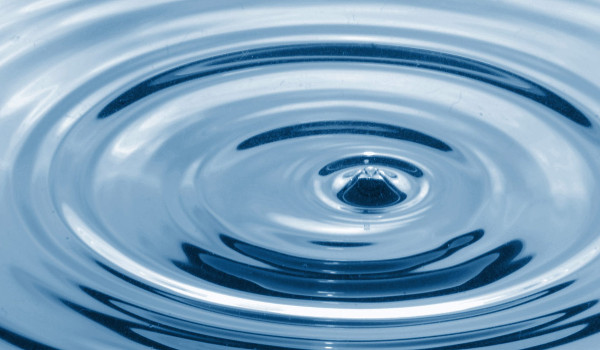
\includegraphics[width=\columnwidth]{img/goccia.jpg}
      \end{figure}
    \end{column}
    \begin{column}{0.3\textwidth}
      \visible<2->{\begin{figure}
        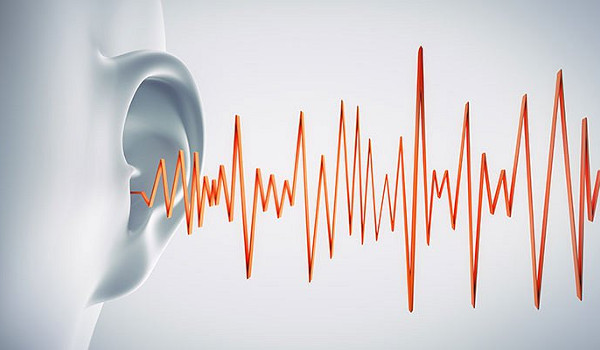
\includegraphics[width=\columnwidth]{img/suono.jpg}
      \end{figure}}
    \end{column}
    \begin{column}{0.3\textwidth}
      \visible<3->{\begin{figure}
        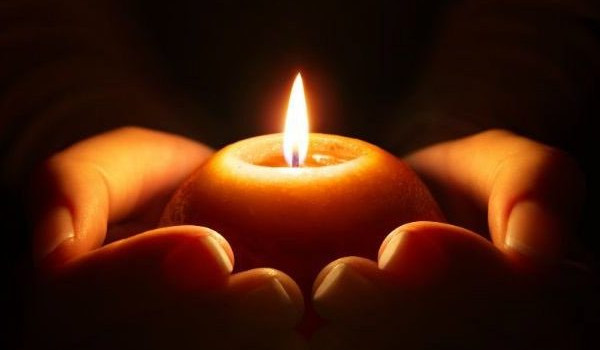
\includegraphics[width=\columnwidth]{img/candela.jpg}
      \end{figure}}
    \end{column}
  \end{columns}
\visible<4>{  \begin{block}{Onda}
    Un'onda è una perturbazione che si propaga trasportando energia ma non materia.\\
    Le onde materiali richiedono un mezzo per propagarsi, le onde elettromagnetiche si propagano anche nel vuoto.
  \end{block}}
\end{frame}

\begin{frame}
  \frametitle{Onde longitudinali e trasversali}
Possiamo distinguere le onde materiali in:
\begin{itemize}
  \item \alert<1>{onde longitudinali}, quando le particelle del mezzo oscillano \alert<1>{parallelamente} al moto dell'onda;\pause
  \item \alert<2>{onde trasversali}, quando le particelle del mezzo oscillano \alert<2>{perpendicolarmente} al moto dell'onda.
  \end{itemize}
  \begin{figure}
        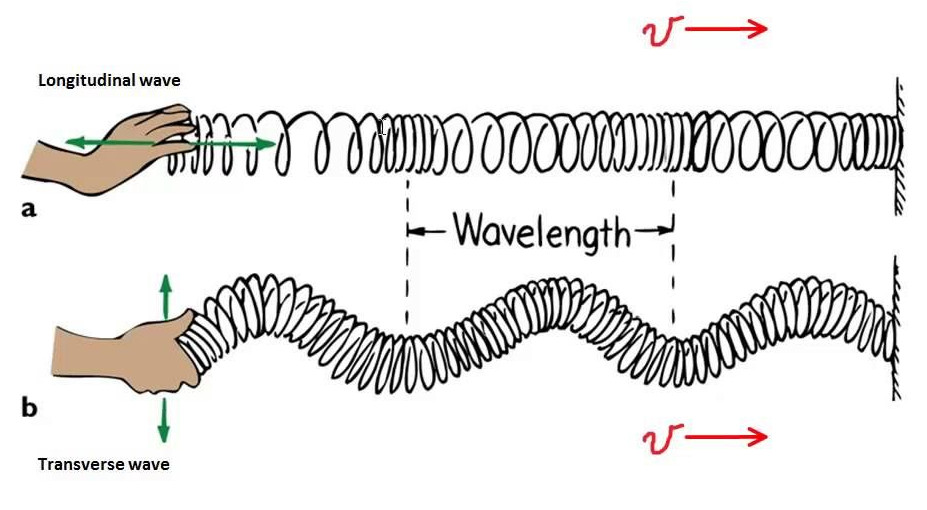
\includegraphics[width=.7\columnwidth]{img/ondalongtrasv.jpg}
      \end{figure}
\end{frame}

\begin{frame}
  \frametitle{Onde elastiche}
Alcune onde si propagano nei mezzi materiali a causa delle proprietà elastiche del mezzo stesso: sono dette \alert<1>{onde elastiche}.\\~\pause\\
Le onde sull'acqua non sono onde elastiche, così come non lo sono le onde radio e la luce.\\~\pause\\
\begin{block}{Grandezza oscillante}
Un'onda è definita dalla grandezza fisica che oscilla durante la sua propagazione.
\end{block}
\end{frame}


\begin{frame}
  \frametitle{Fronti d'onda e raggi}
\begin{block}{Fronte d'onda}
Un fronte d'onda è un insieme di punti in cui la grandezza oscillante dell'onda assume lo stesso valore.
\end{block}\pause
\begin{block}{Raggio}
I raggi sono rette perpendicolari ai fronti d'onda.
\end{block}
\begin{figure}
        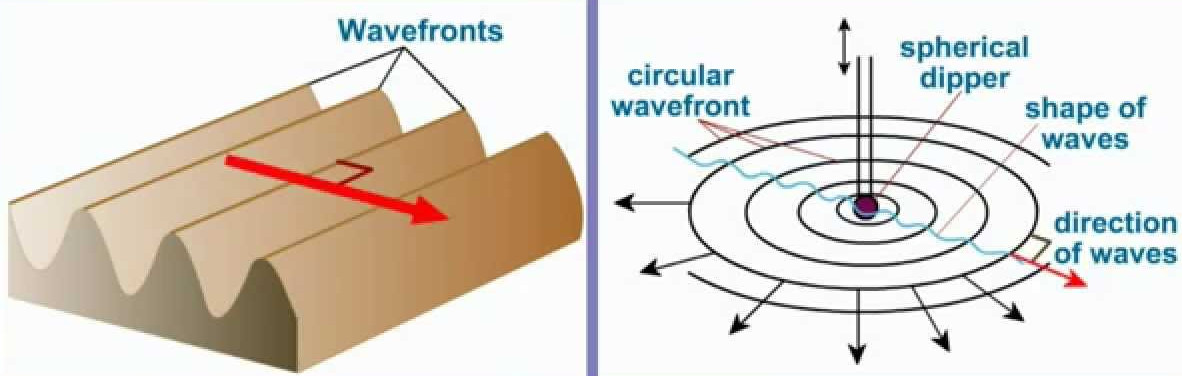
\includegraphics[width=.9\columnwidth]{img/frontidonda.jpg}
      \end{figure}
\end{frame}

\section{Onde periodiche}


\begin{frame}
  \frametitle{Ripetizione di onde}
\begin{block}{Onda periodica}
Un'onda periodica è un'onda che si ripete identica dopo un intervallo di tempo costante.
\end{block}
\begin{figure}
\begin{tikzpicture}[xscale=.4,yscale=1.2]
\node [below] at (6*pi,0) {{\scriptsize $ t $}};
\node [left] at (0,1.5) {{\scriptsize $ y $}};
\draw [->] (-4,0) -- (6*pi,0);
\draw [->] (0,-1.5) -- (0,1.5);
\draw[smooth, red, thick, domain=-4:0*pi] plot (\x, {sin(\x r)});
\draw[smooth, green, thick, domain=-0*pi:2*pi] plot (\x, {sin(\x r)});
\draw[smooth, orange, thick, domain=2*pi:4*pi] plot (\x, {sin(\x r)});
\draw[smooth, blue, thick, domain=4*pi:5.5*pi] plot (\x, {sin(\x r)});
\end{tikzpicture}
\end{figure}
\end{frame}




\begin{frame}
  \frametitle{Caratteristiche spaziali di un'onda}
\begin{figure}
\begin{tikzpicture}[xscale=.4,yscale=1.2]
\node [below] at (4*pi,0) {{\scriptsize $ x $}};
\node [left] at (0,1.5) {{\scriptsize $ y $}};
\node [above] at (1.5*pi,1) {{\scriptsize $ \lambda $}};
\draw [->] (-4,0) -- (4*pi,0);
\draw [|<->|, dashed, thick] (.5*pi,1) -- (2.5*pi,1);
\draw [|<->|, dashed, thick] (2.5*pi,0) -- (2.5*pi,1);
\node [right] at (2.5*pi,.5) {{\scriptsize $ A $}};
\draw [->] (0,-1.5) -- (0,1.5);
\draw[smooth, red, thick, domain=-pi:3.5*pi] plot (\x, {sin(\x r)});
\end{tikzpicture}
\end{figure}
\begin{itemize}
  \item $ \lambda $ = \emph{lunghezza d'onda}, la minima distanza dopo cui un'onda si ripete;
  \item $ A $ = \emph{ampiezza dell'onda}, differenza tra il valore massimo e il valore di equilibrio della grandezza oscillante.
\end{itemize}
\end{frame}


\begin{frame}
  \frametitle{Caratteristiche temporali di un'onda}
\begin{figure}
\begin{tikzpicture}[xscale=.4,yscale=1.2]
\node [below] at (4*pi,0) {{\scriptsize $ t $}};
\node [left] at (0,1.5) {{\scriptsize $ y $}};
\node [above] at (1.5*pi,1) {{\scriptsize $ T $}};
\draw [->] (-4,0) -- (4*pi,0);
\draw [|<->|, dashed, thick] (.5*pi,1) -- (2.5*pi,1);
\draw [->] (0,-1.5) -- (0,1.5);
\draw[smooth, blue, thick, domain=-pi:3.5*pi] plot (\x, {sin(\x r)});
\end{tikzpicture}
\end{figure}
\begin{itemize}
  \item $ T $ = \emph{periodo}, l'intervallo di tempo necessario ad un punto del mezzo materiale a compiere un'oscillazione completa;
  \item $ f $ = \emph{frequenza}, numero di oscillazioni effettuate in $ 1 \, s $. La frequenza di misura in \emph{hertz} ($ Hz $) e vale \colorbox{blue!30}{$ f = \frac{1}{T} $}.
\end{itemize}
\end{frame}


\begin{frame}
  \frametitle{Velocità di propagazione}
  Poiché $ v = \frac{\Delta s}{\Delta t} $ e in un periodo l'onda si propaga di una lunghezza d'onda, vale:
  \begin{center}
  \colorbox{blue!30}{$ v = \dfrac{\lambda}{T} = \lambda f $}
  \end{center}\pause
  
  \centering
  \begin{tabular}{c|c|c}
    \textbf{Onda} & \textbf{Mezzo} & \textbf{Velocità} \\\hline\rule{0pt}{3ex}
    Suono & Aria a $ 20 \,{}^\circ C$ & $ 343 \, \frac{m}{s} $ \\\rule{0pt}{3ex}
    Suono & Aria a $ 0\,{}^\circ C $ & $ 331 \, \frac{m}{s} $ \\\rule{0pt}{3ex}
    Suono & Acqua a $ 20\,{}^\circ C $ & $ 1484 \, \frac{m}{s} $ \\\rule{0pt}{3ex}
    Luce & Vuoto & $ 3 \times 10^8 \, \frac{m}{s} $\\
  \end{tabular}
\end{frame}

\begin{frame}
\frametitle{Esercizi}
\begin{exampleblock}{Onde sul mare (1)}
  \small{In un tratto di mare troviamo delle onde con un periodo di $ 6,0 \, s $ e con una lunghezza d'onda di $ 90 \, m $.

  Calcola:
  \begin{itemize}
    \item la frequenza dell'onda;
    \item la sua velocità di propagazione.
  \end{itemize}  }
\end{exampleblock}

~

\begin{exampleblock}{Onde sul mare (2)}
  \small{Un'onda in acqua si propaga con la velocità di $ 18 \, m/s $ e ha una frequenza di $ 0,18 \, Hz $.
  
  Quanto vale la distanza tra una cresta e una gola dell'onda?\hspace*{\fill}[$ 50 \, m $]}
\end{exampleblock}
\end{frame}



\begin{frame}
\frametitle{Esercizio}
\begin{exampleblock}{Velocità di propagazione}
  \small{Una punta che vibra alla frequenza di $ 50,0 \, Hz $ immersa in una vasca piena d’acqua produce una serie di $ 200 $ onde che si estendono su un tratto di $ 8,40 \, m $, ognuna di ampiezza $ 28,2 \, cm $.
  \begin{itemize}
  \item Calcola la lunghezza d'onda dell'onda.\hspace*{\fill}[$ 4,20 \times 10^{-2} \, m $]
  \item Calcola la velocità di propagazione dell'onda.\hspace*{\fill}[$ 2,10 \, m/s $]
  \end{itemize}}
\end{exampleblock}
\end{frame}


\section{Onde armoniche}


\begin{frame}
\frametitle{Moto armonico}
  Il tipo di oscillazione più semplice è quella data da un \emph{moto armonico}.\\~\pause\\
  \begin{block}{Onda armonica}
    Un'onda si dice armonica quando la grandezza che la definisce oscilla di moto armonico.
  \end{block}
  \visible<3>{\begin{figure}
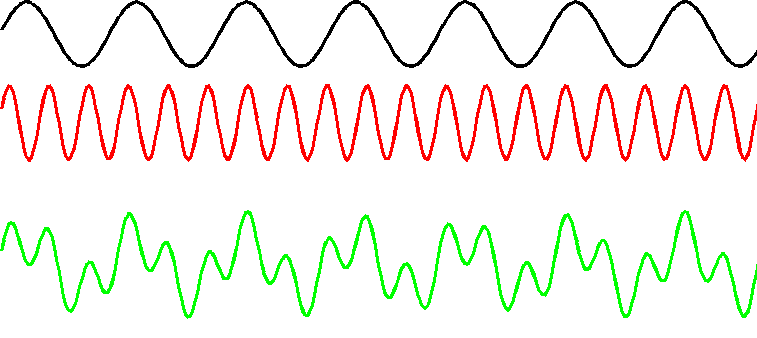
\includegraphics[width=.5\columnwidth]{img/ondearmoniche.png}

Le prime due onde sono armoniche, la terza è solo periodica.
  \end{figure}}
\end{frame}

\begin{frame}
  \frametitle{Leggi delle onde armoniche (1)}
  Scelto un punto di un'onda armonica, la grandezza oscillante in tale punto assumerà valori diversi nel tempo, secondo la legge:
  \begin{center}
  \colorbox{blue!30}{$ y(t) = A \cos \left( \alert<2>{ \dfrac{2\pi}{T}t + \alert<3>{\varphi_0} } \right) = A \cos \left( \alert<4>{\omega} t + \varphi_0 \right) $}
  \end{center}\pause
  \begin{itemize}
    \item la quantità tra parentesi è la \alert<2>{fase} dell'onda;\pause
    \item in $ t=0 \, s $ la fase vale $ \varphi_0 $, che pertanto è la \alert<3>{fase iniziale} dell'onda;\pause
    \item $ \omega $ è la \alert<4>{pulsazione/velocità angolare} del moto armonico che genera l'onda.
  \end{itemize}
\end{frame}



\begin{frame}
  \frametitle{Leggi delle onde armoniche (2)}
  Scelto un istante $ t $ nel tempo, la grandezza oscillante in tale istante assumerà valori diversi nello spazio, secondo la legge:
  \begin{center}
  \colorbox{blue!30}{$ y(x) = A \cos \left( \alert<2>{ \dfrac{2\pi}{\alert<3>{\lambda}}x + \varphi_0 } \right) $}
  \end{center}\pause
  \begin{itemize}
    \item la quantità tra parentesi è ancora la \alert<2>{fase} dell'onda;\pause
    \item \alert<3>{$ \lambda $} è l'analogo spaziale del periodo dell'onda.
  \end{itemize}
\end{frame}


\begin{frame}
  \frametitle{Interpretazione delle formule}
Le leggi che abbiamo visto valgono per tutte le onde armoniche, indipendentemente dal tipo di onda. Ciò che cambia è il \alert{significato della variabile $ y $}:\pause
\begin{itemize}
  \item per il suono è la densità dell'aria;\pause
  \item per le onde elettromagnetiche sono i valori dei campi elettrici e magnetici;\pause
  \item per le onde su una corda è l'altezza raggiunta dalla corda.
\end{itemize}
\end{frame}


\begin{frame}
\frametitle{Esercizio}
\begin{exampleblock}{Dall'equazione ai dati}
  \small{L'oscillazione di un punto di una corda avviene secondo l'equazione:
  \[ y(t) = (0,80 \, m) \cos (2\pi t) \]
  La velocità di propagazione dell'onda è di $ 0,040 \, \frac{m}{s} $.
  \begin{itemize}
  \item Calcola la lunghezza d'onda dell'onda che si propaga nella corda.\hspace*{\fill}[$ 4,0 \times 10^{-2} \, m $]
  \item Costruisci il grafico dell'altezza dell'onda in funzione del tempo per i primi $ 2,00 \, s $.
  \end{itemize}}
\end{exampleblock}
\end{frame}


\section{Interferenza}

\begin{frame}
  \frametitle{Sovrapposizione}
  Che cosa accade quando due o più onde (ad esempio due o più suoni) si propagano contemporaneamente nello stesso mezzo materiale?\\~\pause
  \begin{block}{Principio di sovrapposizione}
    Due o più onde che si propagano nello stesso mezzo generano una perturbazione che è la \alert{somma} delle perturbazioni che ciascuna onda produrrebbe da sola.\pause
    
    Per due onde:
    \begin{center}
    \colorbox{blue!30}{$ y_{tot}(t) = A_1 \cos \left( \omega_1 t + \varphi_1 \right) \alert{+} A_2 \cos \left( \omega_2 t + \varphi_2 \right) $}
    \end{center}
  \end{block}
\end{frame}

\begin{frame}
  \frametitle{Interferenza costruttiva}
  \begin{block}{Interferenza costruttiva}
    Si ha interferenza costruttiva quando gli effetti di due o più onde si rafforzano a vicenda.
  \end{block}\pause
  
  \begin{columns}
\begin{column}{0.5\textwidth}
\begin{center}
Onde in fase
\end{center}
\begin{figure}
\begin{tikzpicture}[xscale=.2,yscale=.6]
\draw [->] (-4,0) -- (3.5*pi,0);
\draw [->] (0,-1) -- (0,1);
\draw[smooth, magenta, thick, domain=-4:3.5*pi] plot (\x, {sin(\x r)});
\end{tikzpicture}

+

\begin{tikzpicture}[xscale=.2,yscale=.6]
\draw [->] (-4,0) -- (3.5*pi,0);
\draw [->] (0,-1) -- (0,1);
\draw[smooth, magenta, thick, domain=-4:3.5*pi] plot (\x, {sin(\x r)});
\end{tikzpicture}
\end{figure}

\end{column}
\begin{column}{0.5\textwidth}
\begin{center}
Onda con ampiezza maggiore
\end{center}
\begin{figure}
\begin{tikzpicture}[xscale=.2,yscale=.6]
\draw [->,white] (-4,-2.4) -- (-4,2.4);
\draw [->] (-4,0) -- (3.5*pi,0);
\draw [->] (0,-2) -- (0,2);
\draw[smooth, purple, thick, domain=-4:3.5*pi] plot (\x, {2*sin(\x r)});
\end{tikzpicture}
\end{figure}

\end{column}
\end{columns}

\end{frame}


\begin{frame}
  \frametitle{Interferenza distruttiva}
    \begin{block}{Interferenza distruttiva}
    Si ha interferenza distruttiva quando gli effetti di due o più onde si annullano a vicenda.
  \end{block}\pause
    \begin{columns}
\begin{column}{0.5\textwidth}
\begin{center}
Onde in opposizione di fase
\end{center}
\begin{figure}
\begin{tikzpicture}[xscale=.2,yscale=.6]
\draw [->] (-4,0) -- (3.5*pi,0);
\draw [->] (0,-1) -- (0,1);
\draw[smooth, magenta, thick, domain=-4:3.5*pi] plot (\x, {sin(\x r)});
\end{tikzpicture}

+

\begin{tikzpicture}[xscale=.2,yscale=.6]
\draw [->] (-4,0) -- (3.5*pi,0);
\draw [->] (0,-1) -- (0,1);
\draw[smooth, violet, thick, domain=-4:3.5*pi] plot (\x, {-sin(\x r)});
\end{tikzpicture}
\end{figure}

\end{column}
\begin{column}{0.5\textwidth}
\begin{center}
Onda nulla
\end{center}
\begin{figure}
\begin{tikzpicture}[xscale=.2,yscale=.6]
\draw [->,white] (-4,-2.4) -- (-4,2.4);
\draw [->] (-4,0) -- (3.5*pi,0);
\draw [->] (0,-2) -- (0,2);
\draw[smooth, purple, thick, domain=-4:3.5*pi] plot (\x, {0*sin(\x r)});
\end{tikzpicture}
\end{figure}

\end{column}
\end{columns}

\end{frame}

\begin{frame}
  \frametitle{Sfasamento (1)}
  L'avere interferenza costruttiva o distruttiva dipende dalla differenza $ |\varphi_2 - \varphi_1| $ tra le fasi delle due onde.{\pause} Per due onde con lo stesso periodo vale che:
  \begin{itemize}
    \item se lo sfasamento vale $ 2k\pi $, con $ k \in \mathbb{Z} $, si ha interferenza costruttiva;\pause
    \item se lo sfasamento vale $ (2k+1)\pi $, con $ k \in \mathbb{Z} $, si ha interferenza distruttiva.\pause
  \end{itemize}
  Detto altrimenti, se le due onde sono sfasate di un numero intero di periodi, allora si avrà interferenza costruttiva; se la differenza sarà maggiore o minore di prima di mezzo periodo, si avrà interferenza distruttiva.
\end{frame}


\begin{frame}
  \frametitle{Sfasamento (2)}
  
\begin{columns}
\begin{column}{0.5\textwidth}

\begin{figure}
Per l'interferenza costruttiva:

~

\begin{tikzpicture}[xscale=.2,yscale=.6]
\draw [->] (-4,0) -- (5.5*pi,0);
\draw [->] (0,-1) -- (0,1);
\draw[smooth, magenta, thick, dashed, domain=-4:0*pi] plot (\x, {sin(\x r)});
\draw[smooth, magenta, thick, dashed, domain=2*pi:5.5*pi] plot (\x, {sin(\x r)});
\draw[smooth, magenta, thick, domain=0:2*pi] plot (\x, {sin(\x r)});
\end{tikzpicture}

~

\begin{tikzpicture}[xscale=.2,yscale=.6]
\draw [->] (-4,0) -- (5.5*pi,0);
\draw [->] (0,-1) -- (0,1);
\draw[smooth, magenta, thick, dashed, domain=-4:2*pi] plot (\x, {sin(\x r)});
\draw[smooth, magenta, thick, dashed, domain=4*pi:5.5*pi] plot (\x, {sin(\x r)});
\draw[smooth, magenta, thick, domain=2*pi:4*pi] plot (\x, {sin(\x r)});
\end{tikzpicture}

$ \Delta\varphi $ = un intero  periodo

\end{figure}


\end{column}
\begin{column}{0.5\textwidth}

\begin{figure}
Per l'interferenza distruttiva:

~

\begin{tikzpicture}[xscale=.2,yscale=.6]
\draw [->] (-4,0) -- (5.5*pi,0);
\draw [->] (0,-1) -- (0,1);
\draw[smooth, purple, thick, dashed, domain=-4:0*pi] plot (\x, {sin(\x r)});
\draw[smooth, purple, thick, dashed, domain=2*pi:5.5*pi] plot (\x, {sin(\x r)});
\draw[smooth, purple, thick, domain=0:2*pi] plot (\x, {sin(\x r)});
\end{tikzpicture}

~

\begin{tikzpicture}[xscale=.2,yscale=.6]
\draw [->] (-4,0) -- (5.5*pi,0);
\draw [->] (0,-1) -- (0,1);
\draw[smooth, purple, thick, dashed, domain=-4:1*pi] plot (\x, {-sin(\x r)});
\draw[smooth, purple, thick, dashed, domain=3*pi:5.5*pi] plot (\x, {-sin(\x r)});
\draw[smooth, purple, thick, domain=1*pi:3*pi] plot (\x, {-sin(\x r)});
\end{tikzpicture}

$ \Delta\varphi $ = mezzo periodo

\end{figure}


\end{column}
\end{columns}
\end{frame}







\end{document}
